% 9.	一家洗衣粉制造公司作新产品试验时,关心洗衣粉泡沫的高度y与搅拌程度x1和洗衣粉用量x2之间的关系,其中搅拌程度从弱到强分为3个水平。试验得到的数据如表13.30。
% 1)	将搅拌程度x1作为普通变量,建立y与x1和x2的回归模型,从残差图上发现问题。
% 2)	将搅拌程度x1视为没有定量关系的3个水平,用0-1变量表示,建立回归模型,与1)比较。从残差图上还能发现什么问题。
% 3)	加入搅拌程度与洗衣粉用量的交互项,看看模型有无改进。

\subsubsection{算法设计}

\paragraph{第(1)问} 将搅拌程度$x_1$作为普通变量,建立$y$与$x_1$和$x_2$的多元线性回归模型为,
\begin{equation}
    y = \beta_0 + \beta_1 x_1 + \beta_2 x_2 + \varepsilon
\end{equation}

在MATLAB中,可使用\texttt{stepwise}命令进行逐步回归,使用\texttt{regress}命令计算多元线性回归。

\paragraph{第(2)问} 为了避免引入定量关系,可用两个变量$(x_{1a},x_{1b})$表达搅拌程度$x_1$,令$(0,0)$表示$x_1=1$,令$(0,1)$表示$x_1=2$,令$(1,0)$表示$x_1=3$,可建立$y$与$x_{1a},x_{1b},x_2$的多元线性回归模型为,
\begin{equation}
    y = \beta_0 + \beta_{1a} x_{1a} + \beta_{1b} x_{1b} + \beta_2 x_2 + \varepsilon
\end{equation}

同样使用\texttt{stepwise}和\texttt{regress}命令求解。

\paragraph{第(3)问} 在第(2)问的基础上,加入搅拌程度与洗衣粉用量的交互项,可建模如下,
\begin{equation}
    y = \beta_0 + \beta_{1a} x_{1a} + \beta_{1b} x_{1b} + \beta_2 x_2 + \beta_{1a2} x_{1a} x_2 + \beta_{1b2} x_{1b} x_2 + \varepsilon
\end{equation}

同样使用\texttt{stepwise}和\texttt{regress}命令求解。

\subsubsection{程序}

请参见附录\ref{sec:ex9_code}。

\subsubsection{计算结果}

\paragraph{第(1)问} 经过逐步回归和最终计算,得到剩余方差$s^2$最小的多元线性回归模型为,
\begin{equation}\label{eq:ex9_x1_linear}
    y = -12.74 + 26.30 x_1 + 3.09 x_2 + \varepsilon
\end{equation}

详细参数如\Cref{tab:ex9_x1_linear},得到的残差图像如\Cref{fig:ex9_x1_rcoplot},从残差图可以看出,当搅拌程度$x_1=2$时,残差均为正,其余情况下,残差均为负。表明将搅拌程度的三个水平定量表达时,泡沫高度$y$与搅拌程度$x_1$的线性程度较差。

\begin{table}[H]
    \centering
    \caption{多元线性回归模型}
    \label{tab:ex9_x1_linear}
    \begin{tabular}{|c|c|c|}
        \hline
        回归系数 & 估计值 & 置信区间\\
        \hline
        \hline
        \(\beta_0\) & -12.7400 & [-29.0268, 3.5468]\\
        \hline
        \(\beta_1\) & 26.3000 & [23.1059, 29.4941]\\
        \hline
        \(\beta_2\) & 3.0867 & [1.2426, 4.9308]\\
        \hline
        \multicolumn{3}{|c|}{$R^2=0.9654, \quad F=167.5754, \quad p=0.0000, \quad s^2=21.4910$}\\
        \hline
    \end{tabular}
\end{table}

\begin{figure}[H]
    \centering
    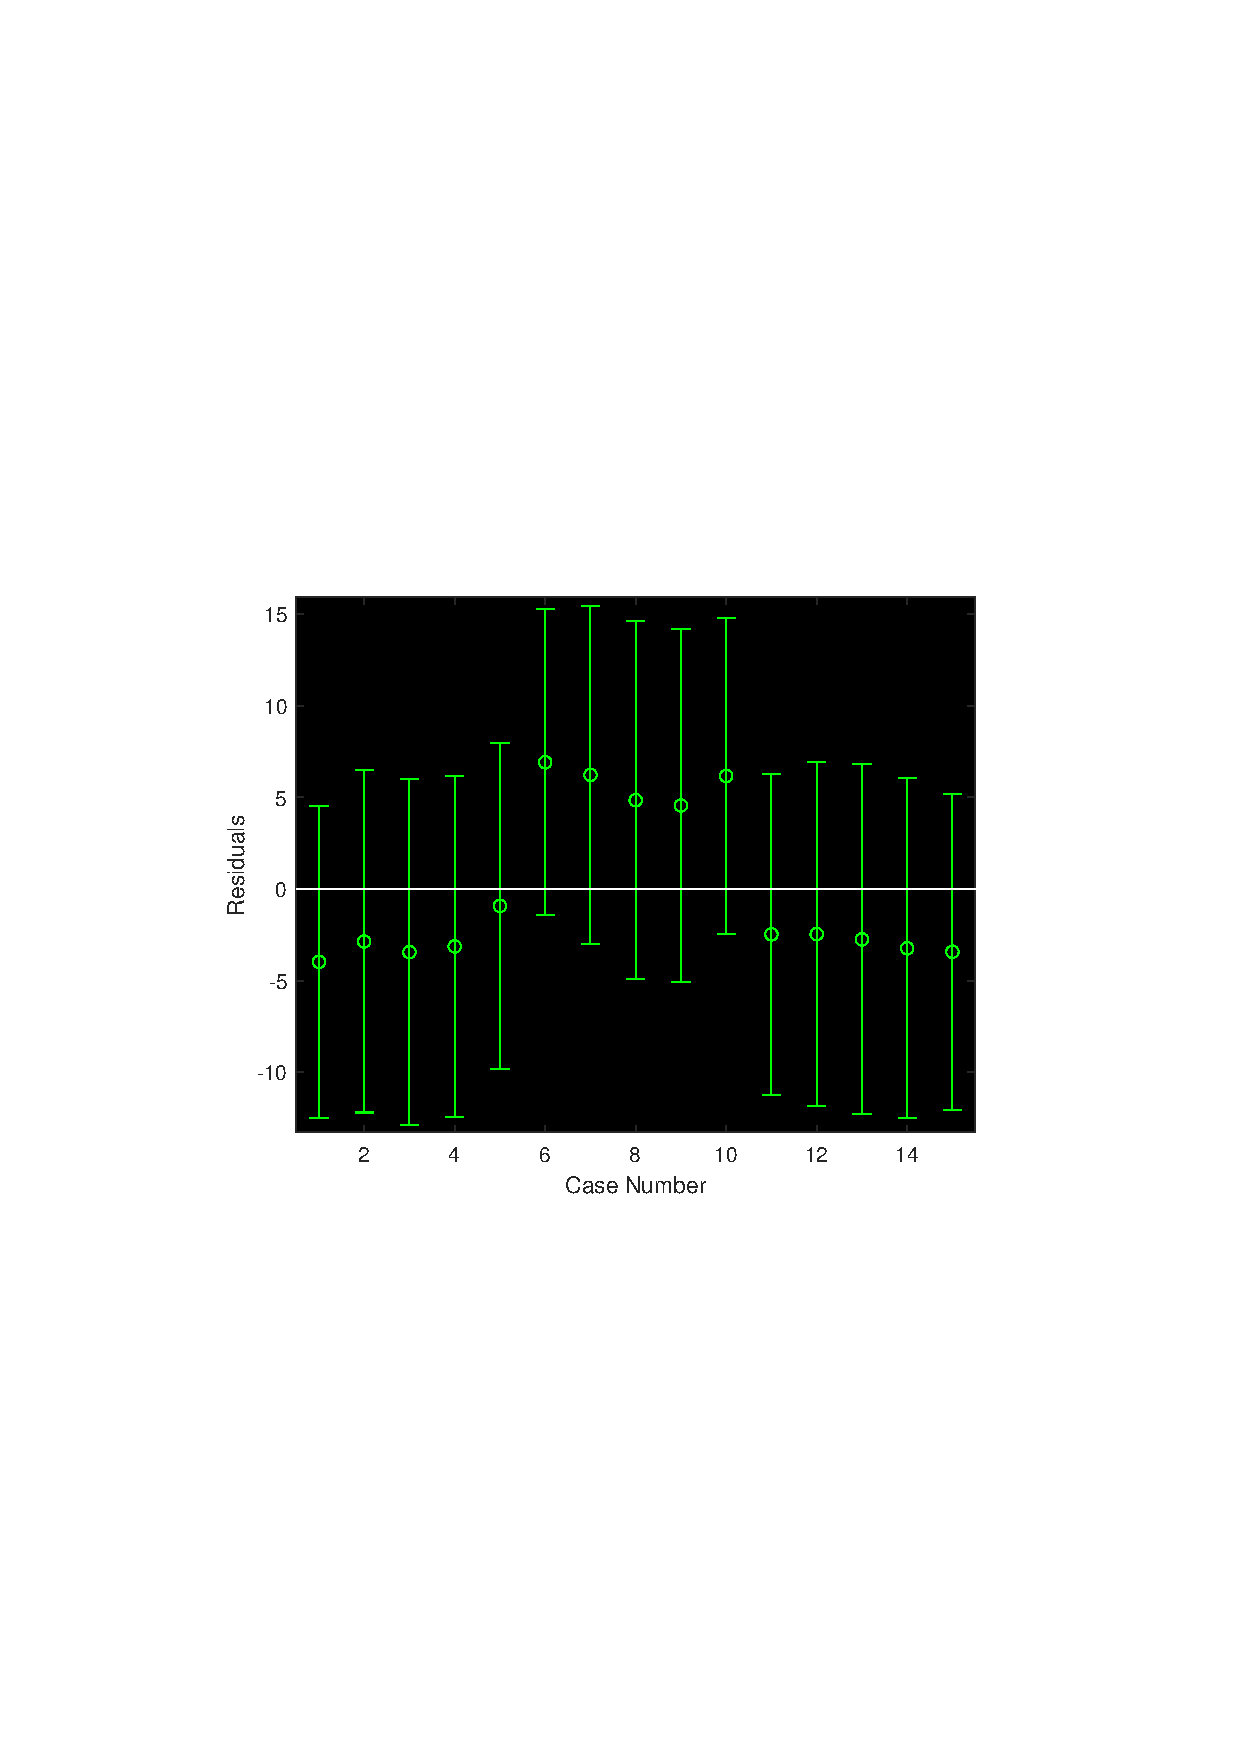
\includegraphics[width=0.8\textwidth,trim={3.09cm 9.295cm 3.09cm 9.295cm},clip]{fig/ex9_x1_rcoplot.pdf}
    \caption{残差图像}
    \label{fig:ex9_x1_rcoplot}
\end{figure}

\paragraph{第(2)问} 经过逐步回归和最终计算,得到剩余方差$s^2$最小的多元线性回归模型为,
\begin{equation}\label{eq:ex9_x1ab_linear}
    y = 10.69 + 52.60 x_{1a} + 34.92 x_{1b} + 3.09 x_2 + \varepsilon
\end{equation}

详细参数如\Cref{tab:ex9_x1ab_linear},与第(1)问相比,剩余方差$s^2$显著下降,决定系数$R^2$也有了明显的提升,显然,该模型的拟合效果比第(1)问更好,原因是避免了不恰当的定量关系,用0-1变量处理不同等级的搅拌程度。

\begin{table}[H]
    \centering
    \caption{多元线性回归模型}
    \label{tab:ex9_x1ab_linear}
    \begin{tabular}{|c|c|c|}
        \hline
        回归系数 & 估计值 & 置信区间\\
        \hline
        \hline
        \(\beta_0\) & 10.6867 & [7.4475, 13.9259]\\
        \hline
        \(\beta_{1a}\) & 52.6000 & [51.2588, 53.9412]\\
        \hline
        \(\beta_{1b}\) & 34.9200 & [33.5788, 36.2612]\\
        \hline
        \(\beta_2\) & 3.0867 & [2.6995, 3.4738]\\
        \hline
        \multicolumn{3}{|c|}{$R^2=0.9986, \quad F=2675.4529, \quad p=0.0000, \quad s^2=0.9282$}\\
        \hline
    \end{tabular}
\end{table}

得到的残差图如\Cref{fig:ex9_x1ab_rcoplot},从残差图可以看出,第5个数据是一个异常点,需要进行剔除。

\begin{figure}[H]
    \centering
    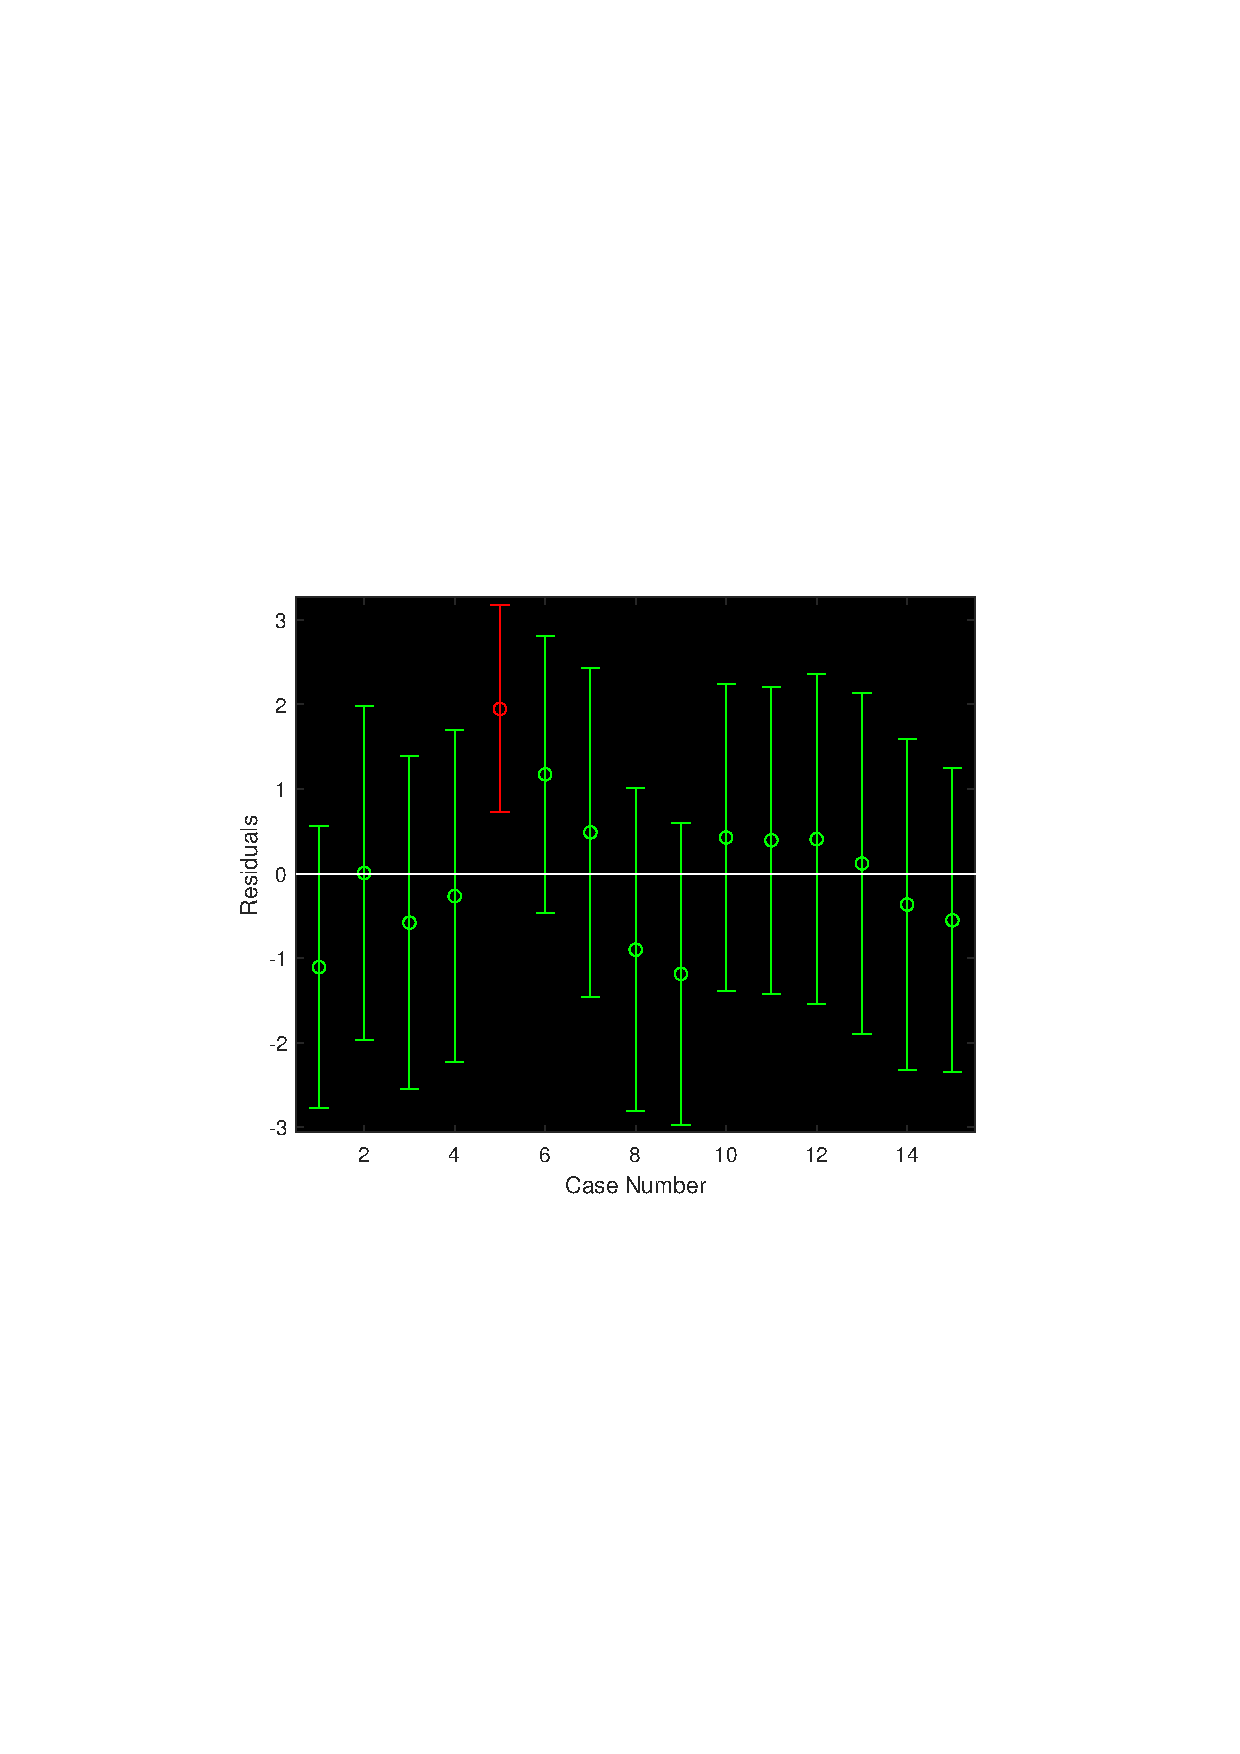
\includegraphics[width=0.8\textwidth,trim={3.09cm 9.295cm 3.09cm 9.295cm},clip]{fig/ex9_x1ab_rcoplot.pdf}
    \caption{残差图像}
    \label{fig:ex9_x1ab_rcoplot}
\end{figure}

剔除所有异常点后,模型修正为,
\begin{equation}
    y = 11.66 + 53.18 x_{1a} + 35.50 x_{1b} + 2.89 x_2 + \varepsilon
\end{equation}

此时残差图如\Cref{fig:ex9_x1ab_rcoplot_no_outlier}。

\begin{figure}[H]
    \centering
    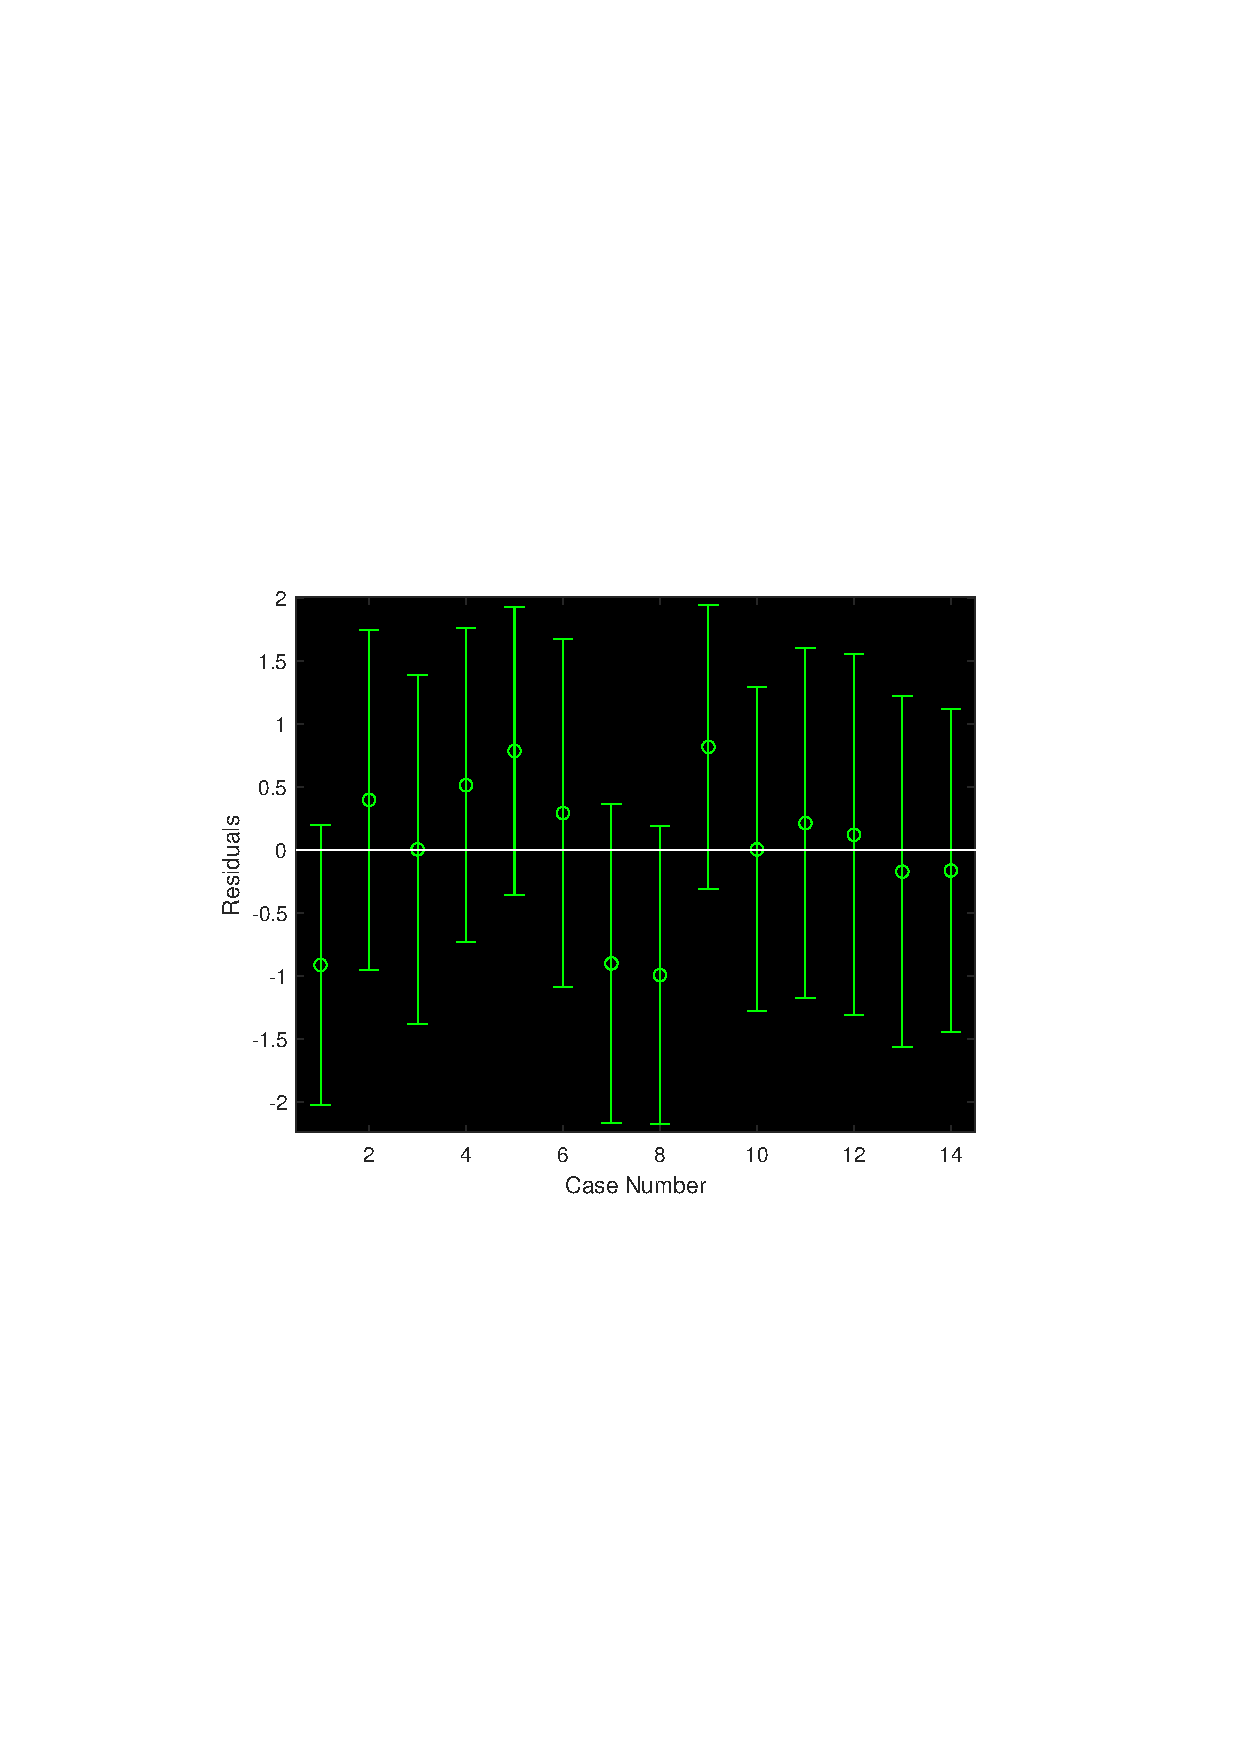
\includegraphics[width=0.8\textwidth,trim={3.09cm 9.295cm 3.09cm 9.295cm},clip]{fig/ex9_x1ab_rcoplot_no_outlier.pdf}
    \caption{残差图像}
    \label{fig:ex9_x1ab_rcoplot_no_outlier}
\end{figure}

\paragraph{第(3)问} 经过计算,得到剩余方差$s^2$最小的多元线性回归模型为,
\begin{equation}\label{eq:ex9_interact}
    y = 6.02 + 59.40 x_{1a} + 42.12 x_{1b} + 3.67 x_2 -0.85 x_{1a} x_2 -0.90 x_{1b} x_2 + \varepsilon
\end{equation}

详细参数如\Cref{tab:ex9_interact},可见,引入交互项后,剩余方差$s^2$和决定系数$R^2$有了进一步改善,模型的拟合效果更好。

\begin{table}[H]
    \centering
    \caption{带有交互项的回归模型}
    \label{tab:ex9_interact}
    \begin{tabular}{|c|c|c|}
        \hline
        回归系数 & 估计值 & 置信区间\\
        \hline
        \hline
        \(\beta_0\) & 6.0200 & [1.6478, 10.3922]\\
        \hline
        \(\beta_{1a}\) & 59.4000 & [53.2167, 65.5833]\\
        \hline
        \(\beta_{1b}\) & 42.1200 & [35.9367, 48.3033]\\
        \hline
        \(\beta_2\) & 3.6700 & [3.1318, 4.2082]\\
        \hline
        \(\beta_{1a2}\) & -0.8500 & [-1.6111, -0.0889]\\
        \hline
        \(\beta_{1b2}\) & -0.9000 & [-1.6611, -0.1389]\\
        \hline
        \multicolumn{3}{|c|}{$R^2=0.9993, \quad F=2634.4605, \quad p=0.0000, \quad s^2=0.5660$}\\
        \hline
    \end{tabular}
\end{table}

\subsubsection{结果分析}

从\Cref{eq:ex9_x1_linear}可以看出,$x_1,x_2$的回归系数均为正数,表明泡沫高度$y$与搅拌程度$x_1$和洗衣粉用量$x_2$均呈正相关,这与生活经验相符。

从\Cref{eq:ex9_x1ab_linear}可以看出,弱搅拌程度对泡沫高度的贡献为0,中等搅拌程度的贡献为34.92,强搅拌程度的贡献为52.60,并不是严格的线性关系,因此,将三个等级的搅拌程度定量为$x_1=1,2,3$并不能表达出这种关系,而应当定量为$x_1=0,34.92,52.60$,这样就能得到与0-1变量相同的结果。然而,这是求解之后才得到的定量方法,在求解之前,使用0-1变量来处理会更合适。

\subsubsection{结论}

将搅拌程度作为普通变量时,回归模型为\Cref{eq:ex9_x1_linear},残差图上,中等搅拌程度的残差与其他情况明显不同。

将搅拌程度视为没有定量关系的3个水平,用0-1变量表示时,回归模型为\Cref{eq:ex9_x1ab_linear},拟合效果得到了明显改善,但残差图上存在异常点。

加入搅拌程度与洗衣粉用量的交互项,回归模型为\Cref{eq:ex9_interact},效果更好。
